% change the aspect ratio to 169 for 16:9 aspect ratio
% otherwise remove option completely for 3:2 ratio.
\documentclass[aspectratio=169]{beamer}
\usepackage[utf8]{inputenc}
\usepackage{amsmath}
\usepackage{amsfonts}
\usepackage{graphicx}


\usetheme{CambridgeUS}

\useinnertheme{rectangles}

% Depending on whether you want dark or light
% theme you can change the style file, 
% drexel-light.tex for light theme and
% drexel-dark.tex for dark theme
\definecolor{drylo}{RGB}{255, 198, 0}
\definecolor{drybl}{RGB}{0,47,108}
 
\definecolor{drblk}{RGB}{0,0,0} 


\setbeamercolor{title}{fg=drybl,bg=drylo}
\setbeamercolor{subtitle}{fg=drybl,bg=drylo}
\setbeamercolor{frametitle}{fg=drybl,bg=drylo!70}
\setbeamercolor{section in head/foot}{bg=drylo}
\setbeamercolor{section in head/foot}{fg=drybl}
\setbeamercolor{subsection in head/foot}{bg=drybl}
\setbeamercolor{author in head/foot}{bg=drylo}
\setbeamercolor{author in head/foot}{fg=drybl}
\setbeamercolor{date in head/foot}{fg=white,bg=drblk}
\setbeamercolor{title in head/foot}{fg=drylo,bg=drybl}

\setbeamercolor{local structure}{fg=drylo,bg=drybl}


\author{Sean C. Lewis}
\title{Galaxies and Stars: Bridging the Expanse}

\date{\today} 
\subject{Physics} 

% depending on dark or light theme use _black or _white pdf for drexel logo.
% These logos are obtained from https://drexel.edu/identity/drexel/logotypes/


% Two graphics side by side
%\titlegraphic{%
%    \hfill
%   
\includegraphics[height=0.7cm]{../images/Drexel_horizontal_black.pdf}%
%    \hfill%
%    
\includegraphics[height=1cm]{../images/EXO_logo.pdf}%
%}

%%%%% Only Drexel
\titlegraphic{%
    %\hfill
    
\includegraphics[height=0.7cm]{../images/Drexel_horizontal_black.pdf}%
    %
\includegraphics[height=0.7cm]{../images/Drexel_horizontal_white.pdf}%
}


\begin{document}

\titlepage

\section{Background}
%
\begin{frame}{Torch}{And Its Next Steps}
    \begin{itemize}
        \item Couples N-body, stellar evolution, and feedback in \texttt{AMUSE} \\ with self-gravitating magnetized gas in MHD code \texttt{FLASH}.
        \item []
        \item Resolved dynamics of stars and gas; study star cluster formation within collapsing GMCs.
    \end{itemize}
\end{frame}




\begin{frame}{Torch}{And Its Next Steps}
    \begin{columns}
        \begin{column}{0.42\textwidth}
            \begin{figure}[h!]
                \centering
                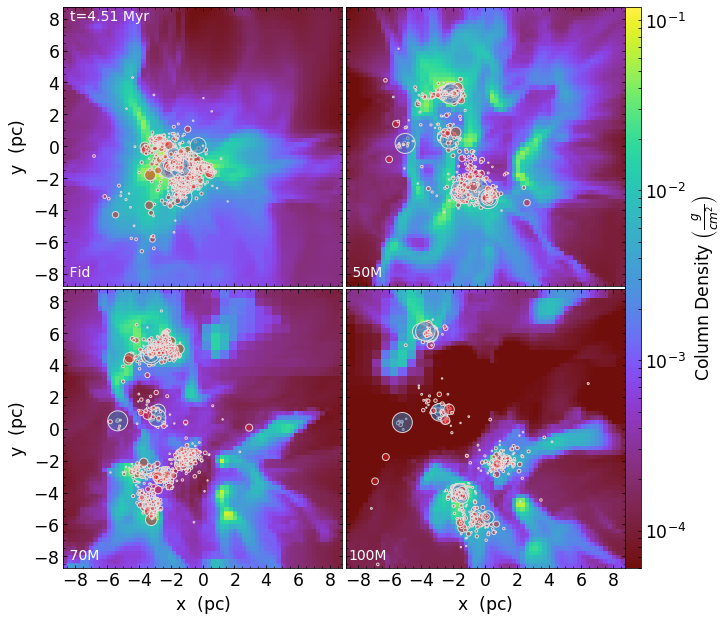
\includegraphics[width=\linewidth]{../images/all_runs_density_grid_time_labels.png} \\
                Lewis et al. (in prep)
                \label{fig:jwst}
            \end{figure}
        \end{column}
        \begin{column}{0.4\textwidth}
            %
            \begin{figure}[h!]
                \centering
                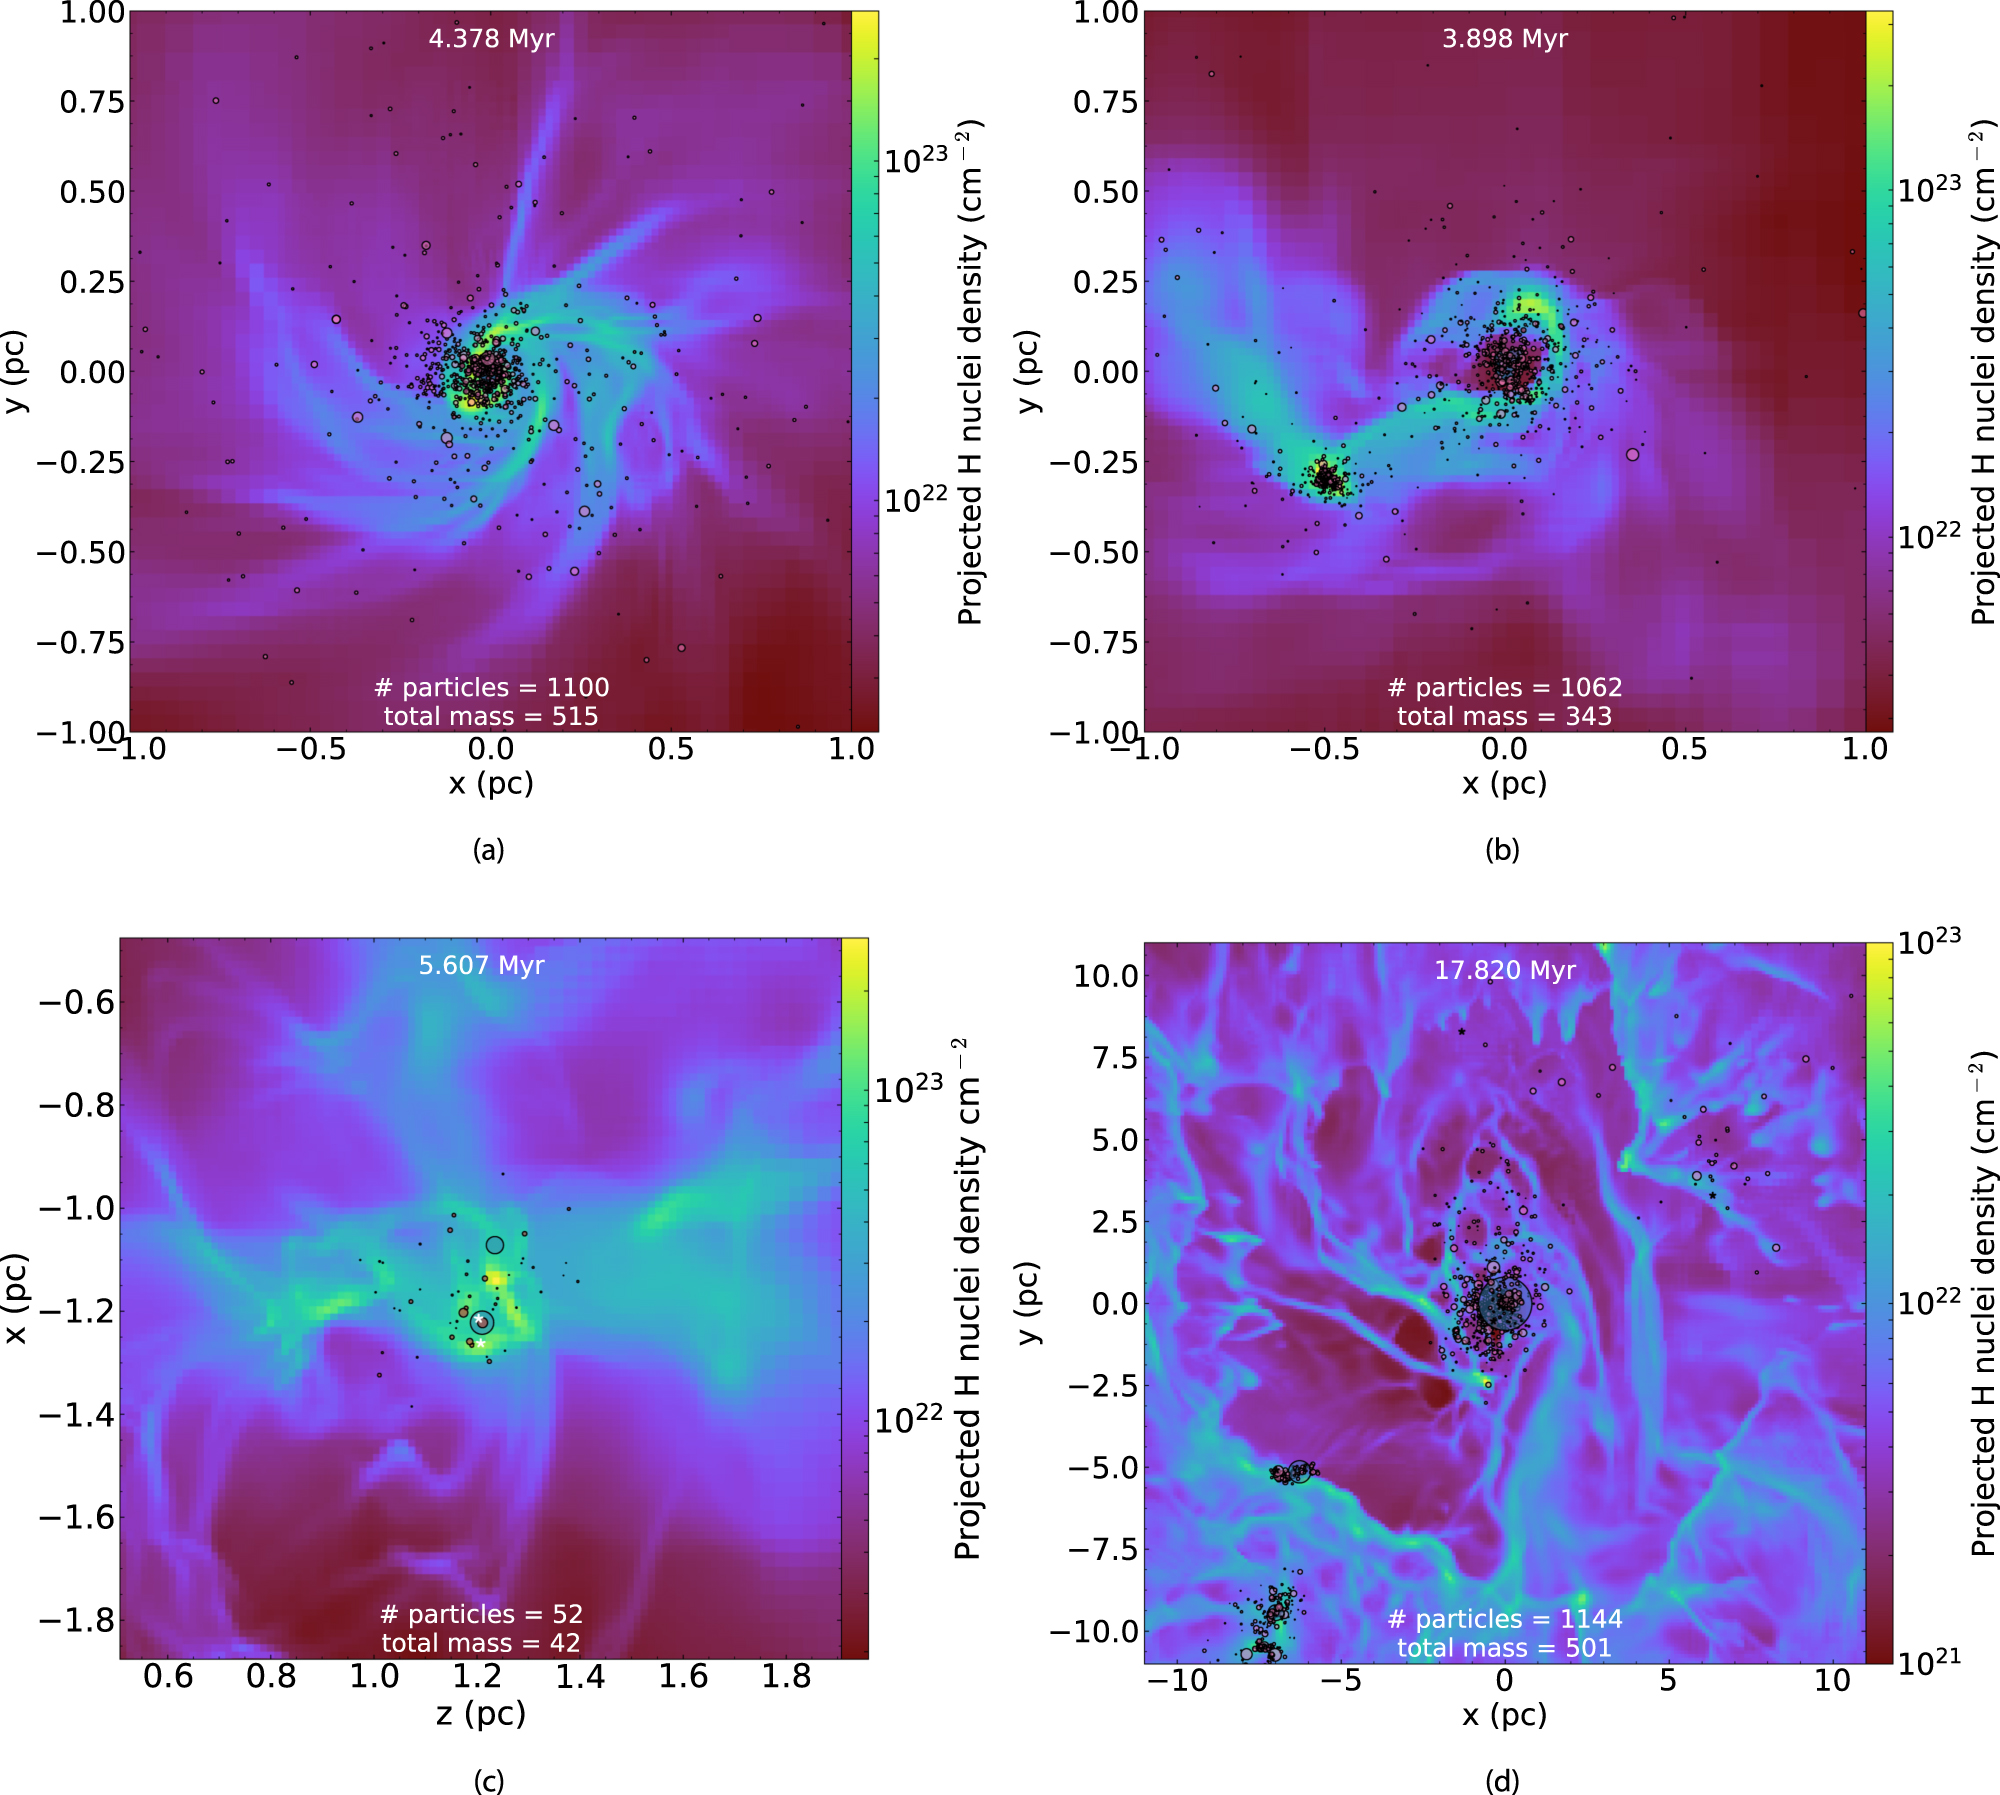
\includegraphics[width=\linewidth]{../images/josh_density_grid.jpeg} \\
                Wall et al. 2020
                \label{fig:torch}
            \end{figure}
        \end{column}
    \end{columns}
\end{frame} 
%
%
%
%
%
\begin{frame}{Clouds in Reality and... Not}{}
    \begin{columns}
        \begin{column}{0.35\textwidth}
            \begin{figure}[h!]
                \centering
                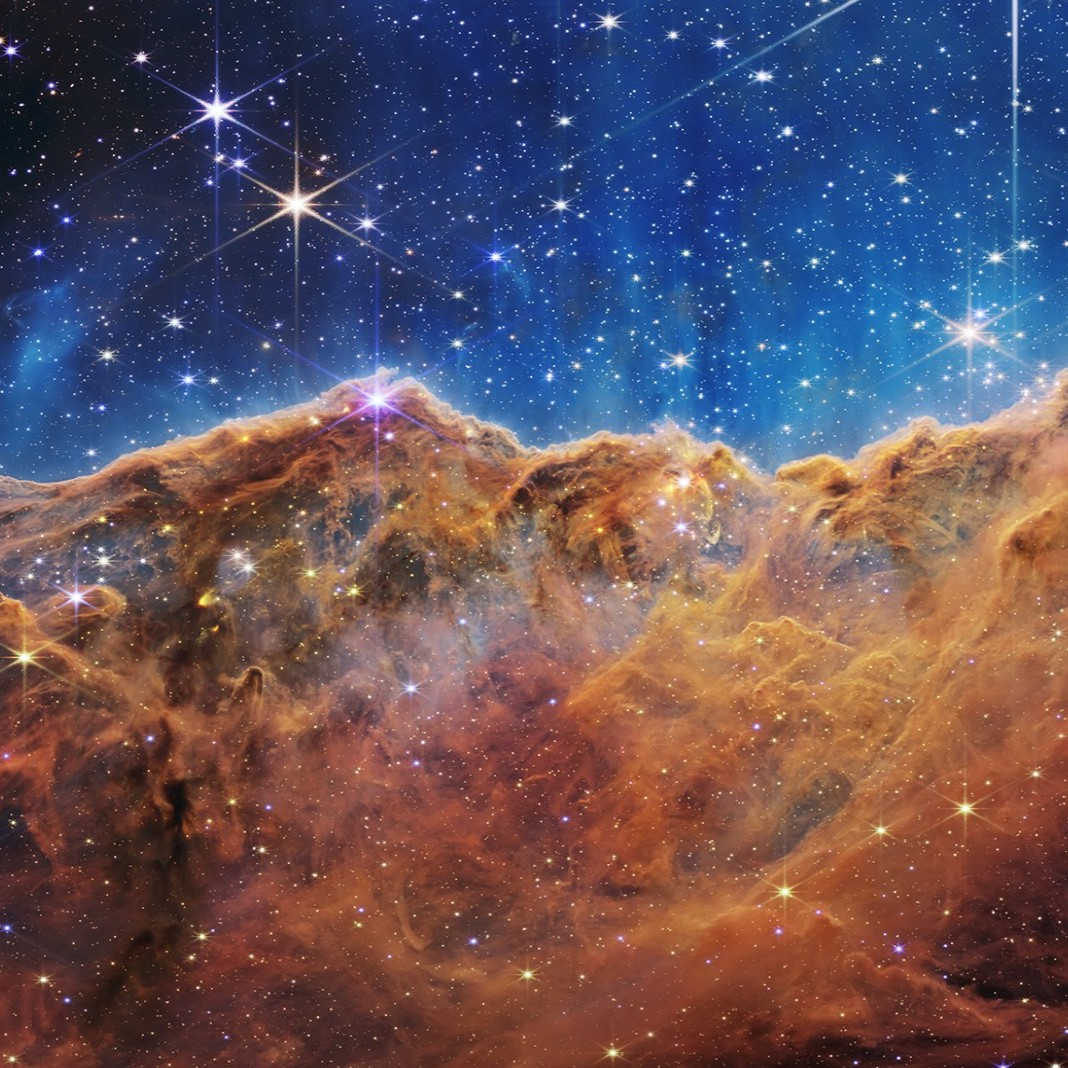
\includegraphics[width=\linewidth]{../images/jwst.jpg} \\
                NASA; Carina Nebula
                \label{fig:jwst}
            \end{figure}
        \end{column}
        \begin{column}{0.35\textwidth}
            %
            \begin{figure}[h!]
                \centering
                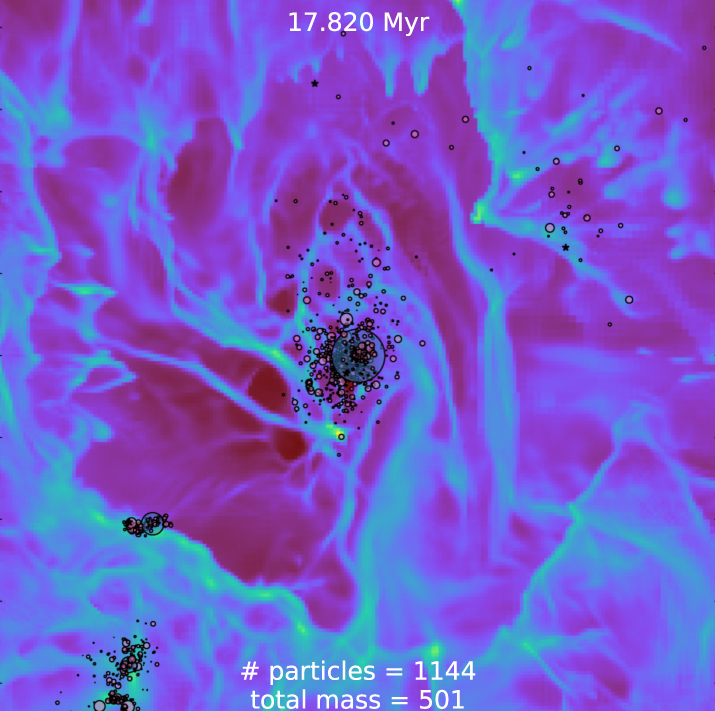
\includegraphics[width=\linewidth]{../images/josh_torch_run.jpeg} \\
                Wall et al. 2020
                \label{fig:torch}
            \end{figure}
        \end{column}
    \end{columns}
\end{frame} 
%
%
%
%
%
\begin{frame}{The Big Problems}{Resolution \& Initial Conditions}
    \begin{itemize}
        \item Self consistent galactic scale simulations with resolution down to sub-tenth parsec scales and include Nbody individual stellar dynamics and individual stellar feedback all at once? A little tough.
        \item []
        \item []
    \end{itemize}
\end{frame}
%
%
%
%
% 
\begin{frame}{The Big Problems}{Resolution \& Initial Conditions}
    \begin{itemize}
        \item Self consistent galactic scale simulations with resolution down to sub-tenth parsec scales and include Nbody individual stellar dynamics and individual stellar feedback all at once? A little tough.
        \item []
        \item Creating our own isolated clouds from scratch? ``Creative liberties..."
        % Like ignoring the galactic environment, starting from spherical or cylindrical conditions.
    \end{itemize}
\end{frame}
%
%
%
\section{Motivation}
%
%
%
%
\begin{frame}{Stars From ``Realistic" Clouds}{}
    \begin{itemize}
        \item Clouds that formed under the influence of galactic dynamics.
        \item []
        \item Track dynamics and feedback of individual stars.
        \item []
        \item High resolution to quantify star-gas interactions.
        % With Torch, we can already do the last two points.
        % So what we really need are some clouds from galactic simulations
    \end{itemize}
\end{frame}
%
%
%
\section{Methods}
%
%
% 
\begin{frame}{Clouds from Galactic Simulations}
	\begin{figure}[h!]
                \centering
                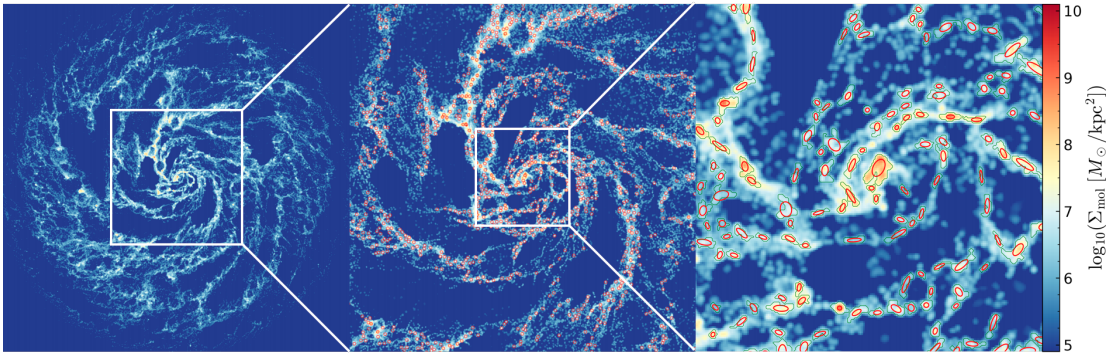
\includegraphics[width=\linewidth]{../images/AREPO_galaxy.png} \\
                GMC identification [Li, H. et al. 2020]
                \label{fig:arepo_galaxy}
	\end{figure}
	% Also have Cloud-Factory Rowen Smith (2019)
\end{frame}
%
%
%
%
%
\begin{frame}{From AREPO to FLASH} {(1st attempt)}
    \begin{columns}
        \begin{column}{0.35\textwidth}
            \begin{figure}[h!]
                \centering
                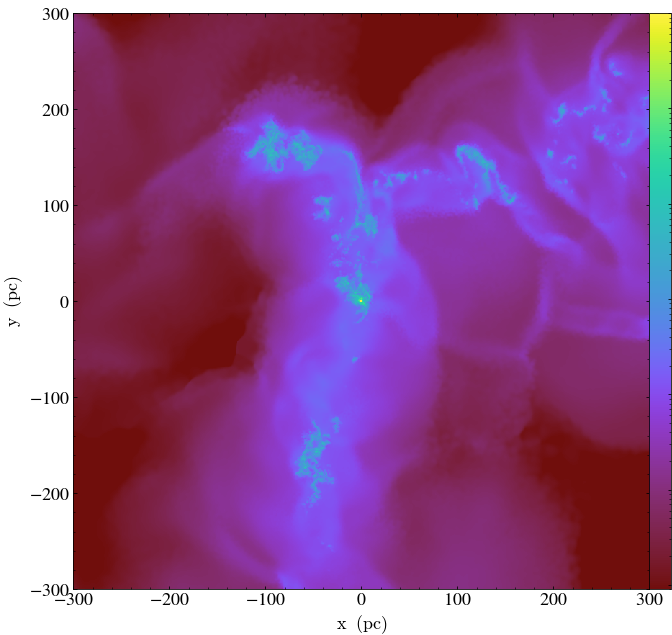
\includegraphics[width=\linewidth]{../images/AREPO_cloud.png} \\
                Cloud from raw AREPO data \\
                -
                \label{fig:voronoi_example}
            \end{figure}
        \end{column}
        \begin{column}{0.35\textwidth}
            %
            \begin{figure}[h!]
                \centering
                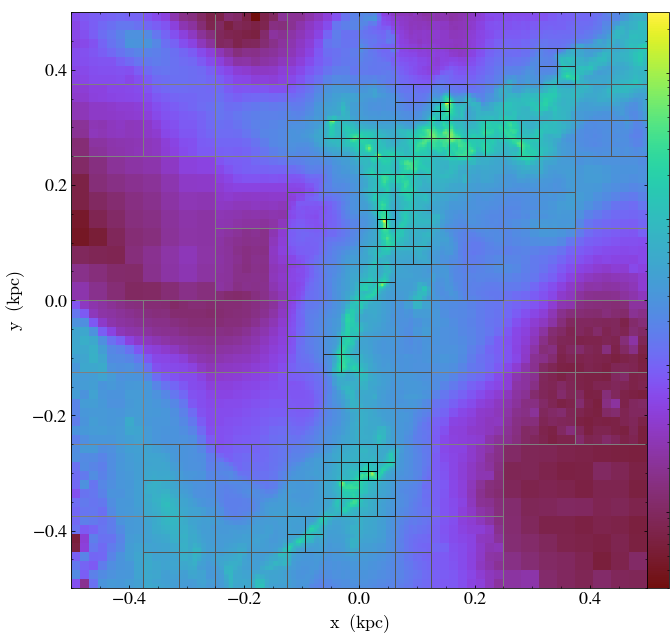
\includegraphics[width=\linewidth]{../images/cloud_in_cell_projection_lvl8.png} \\
                Cloud-in-cell mapping onto AMR FLASH grid
                \label{fig:amr_example}
            \end{figure}
        \end{column}
    \end{columns}
\end{frame} 
%
%
%
%
%
\begin{frame}{Voronoi Mesh to AMR Grid} %{Subtitle not required in this slide}
    \begin{columns}
        \begin{column}{0.39\textwidth}
            \begin{figure}[h!]
                \centering
                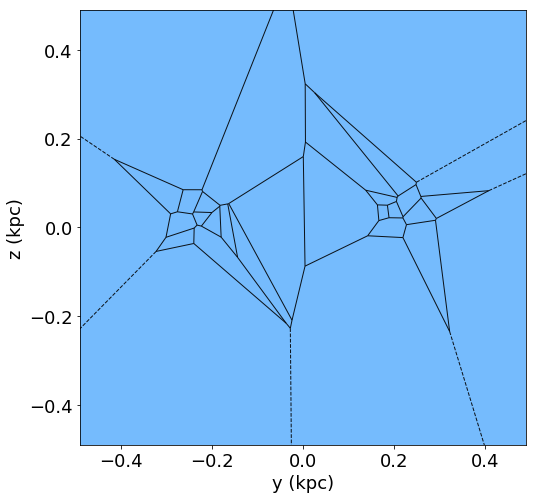
\includegraphics[width=\linewidth]{../images/voronoi_stats.png}
                \caption{Voronoi mesh from 20 points}
                \label{fig:voronoi_example}
            \end{figure}
        \end{column}
        \begin{column}{0.37\textwidth}
            %
            \begin{figure}[h!]
                \centering
                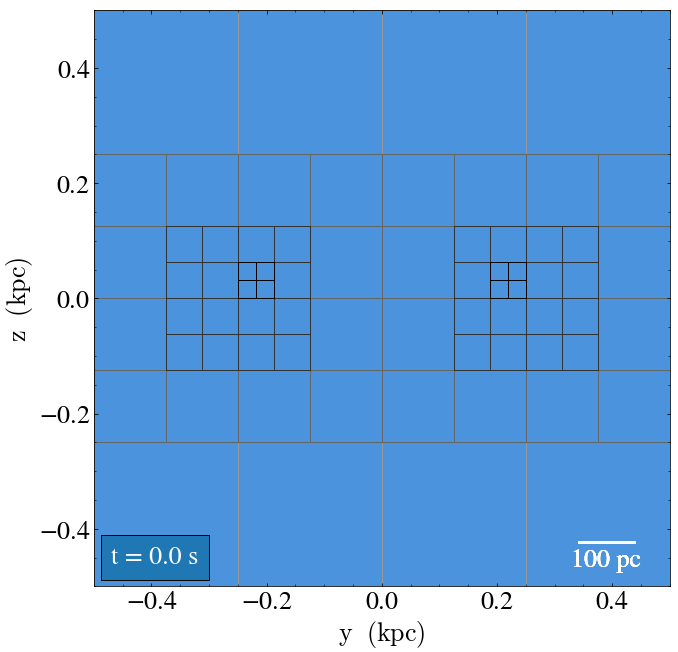
\includegraphics[width=\linewidth]{../images/amr_stats.png}
                \caption{AMR grid from 20 points}
                \label{fig:amr_example}
            \end{figure}
        \end{column}
    \end{columns}
\end{frame} 
%
%
%
%
%
\begin{frame}{VorAMR: Logic path}
	\begin{figure}[h!]
                \centering
                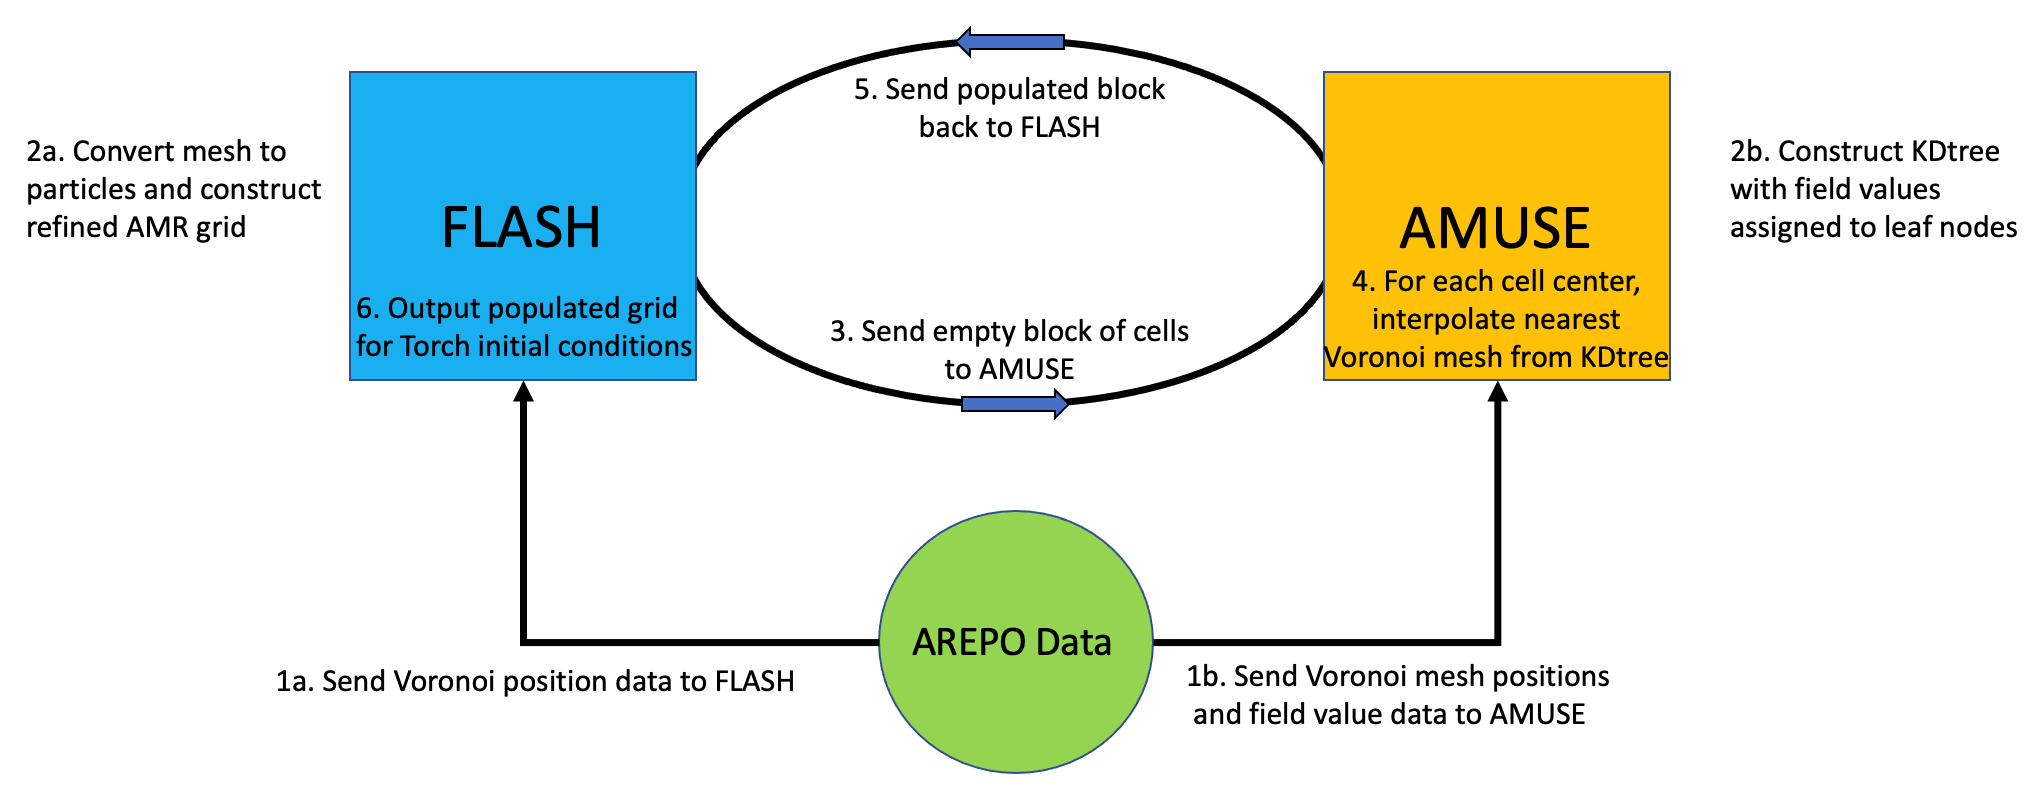
\includegraphics[width=\linewidth]{../images/voramr_logic.png} \\
                \label{fig:voramr_logic}
	\end{figure}
\end{frame}
%
%
%
%
%
% Conversion from Voronoi to AMR grid also allows for better visualizations in yt (which approximates voronoi mesh as sph kernels)
\begin{frame}{VorAMR: The Big Wins}{}
    \begin{itemize}
    	\item Significantly expands Torch's horizon and "completes" Torch.
	\item []
    	\item Opens wide avenue of collaboration; code bases do not have to be exclusive! 
	\item []
	\item More accurate visualizations (no more estimating Voronoi meshes as SPH kernels in \texttt{yt}).
        % With Torch, we can already do the last two points.
        % So what we really need are some clouds from galactic simulations
    \end{itemize}
\end{frame}

\end{document}

